\chapter{Variable Precision Floating Point Representation in Memory}
\label{sec:mem_format}

This document describes the representation of floating point reals for use by the VRP when reading and writing data in memory.
The format is strongly based on IEEE 754 extendable formats as defined in the 2008 standard document \cite{IEEE754}.
For consistency, we use notations from the standard.

This chapter does not cover the internal representation of numbers within the Xvpfloat registers (see Section~\ref{sec:vpregs} instead).

% -----------------------------------------------
\section{Key Parameters}

\subsection{Format parameters}
The extendable format is fully defined by 3 parameters: $b$, $p$ and $w$:
\begin{itemize}[topsep=0pt]
\item $b$ is the radix, $b=2$ in our case.
\item $p$ is the number of digits in the significand (precision) . \\
  note that only $t=p-1$ bits are explicit. The first bit of the significand is implicit and is deduced from the exponent.
\item $w$ is the number of bits of the exponent, from which we derive:
  \begin{itemize}[topsep=0pt]
  \item[$\bullet$]  $emax$ = the maximum exponent $e=2^{{w-1}}-1$
  \item[$\bullet$]  $emin$ = the minimum exponent $e=1-emax$ .
  \end{itemize}
The bit size of a scalar is given by $k=w+p$.
\end{itemize}

\paragraph{Important note:} An extendable precision format is defined under user control with 2 parameters chosen independently : precision $p$ and range $emax$ (or alternatively $w$ ).
The user may choose to comply with an interchange format instead: in that particular case, the format is defined with only one parameter (eg its global size), and the other parameters $p$ and $emax$ are given by explicit formulas in Table 3.5 - Binary interchange format parameters of the norm \cite{IEEE754}.
Specifically, the exponent bit length is given by $round(4*log2(k))-13$. 
For example, limiting exponent size to 18 bits limits $k$ to value 232.

\subsection{Platform specific limits and features}

The Xvpfloat extension has its own limits and features, which are orthogonal to
the standard specifications (IEEE 754-2008), but meaningful for developing and using the platform.

\begin{itemize}[topsep=0pt]
\item Radix: the platform only supports radix 2 numbers.
\item Exponent size ($w$): the platform supports up to IEEE\_Esize\textsubscript{MAX} bits of exponent.
\item Scalar bit size ($k$): the size of any scalar number must be aligned on a byte boundary (i.e. multiple of 8 bits) in the limit of BYS\textsubscript{MAX} bytes.
This constraint reduces the choice of possible expandable formats, but covers the interchange formats.
Thus even though $k$ is provided in bits in BIS parameters, IEEE754-2008 strict compatibility is obtained only with $k^{aligned} = k = 8 \times bys$.
\item Significand size ($p$): the platform supports from as low as three bits of significand \footnote{The minimal value of 3 is related to the standard itself: in addition to the virtual leading '1', at least 2 bits are necessary for disambiguating Inf from Nan.} up to IEEE\_Msize\textsubscript{MAX} bits of significand.
However, significand size will be deduced from exponent and scalar bit size with the formula: $p=k-w$.
Special case arise when $k^{aligned} \neq k=w+p$ for alignement reasons.
In this case, padding is inserted in least significant bits of the mantissa when storing to memory, and those bits are ignored when reading from memory.
\item Endianness : the platform uses little endianness for storing floating point numbers.
This means that the least-significant byte at stored at the smallest address.
\end{itemize}

Table \ref{tab:ieee-sizes} reports the maximum and minimum values for the $w$,
$p$ and, consequently, the $k$ parameters:
\begin{table}[htbp]
\centering
\begin{tabular}{c|c|c}
                           & min size {[}bit{]} & \multicolumn{1}{l}{max sizes {[}bit{]}} \\ \hline
w                          & 1                  & \multicolumn{1}{c|}{18}                 \\ \hline
p                          & 3                  & \multicolumn{1}{c|}{513}                \\ \hline
k                          & 4                  & \multicolumn{1}{c|}{531}                \\ \hline
k\textsuperscript{aligned} & 8                  & \multicolumn{1}{c|}{536}                \\ \cline{2-3}
\end{tabular}
\caption{Constraints on the format fields for Xvpfloat.}
\label{tab:ieee-sizes}
\end{table}

Starting from the maximum size constraints, since $k=w+p$, it is possible to
obtain the
maximum value for $k$. In particular:
\begin{itemize}[topsep=0pt]
    \item $k_{max}$ = $w_{max} + p_{max}$ = 531 bits.
\end{itemize}
For byte alignement reasons, $k^{aligned}_{max}$ is rounded up to 536 bits, which equals 67 bytes to load/store at most.

In case $k > IEEE\_Esize_{MAX}+IEEE\_Msize_{MAX}$, zero-padding is inserted.
The padding is done by adding a number of zeros, $nz$, starting from the least-significant
bit of the significand $d_{p}$, to $d_{p+nz-1}$, Figure \ref{ieee:structure}, with $nz$ = $k -
(1+IEEE\_Esize_{MAX}+IEEE\_Msize_{MAX})$
% -----------------------------------------------
\section{Binary Encoding}

\subsection{Endianness}

IEEE 754 floating-point standard does not specify endianness.
However Xvpfloat assumes little endian binary representation of IEEE-754 format.

\subsection{Structure}
Representations of floating-point data in the binary interchange formats are encoded in k bits in the following three fields ordered as shown below:
\begin{figure}[h!]
  \centering
  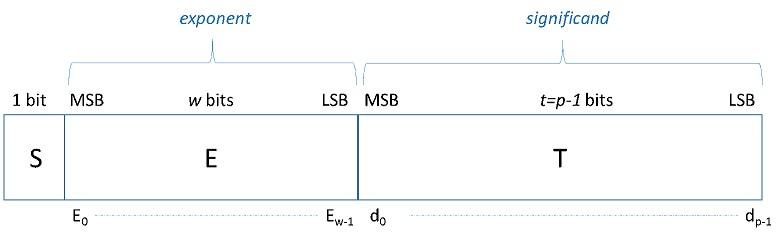
\includegraphics[scale=0.5]{format-small}
  \caption{IEEE binary format structure.}
  \label{ieee:structure}
\end{figure}

% -----------------------------------------------
\section{Representation Semantics}

\subsection{Real Values}
Most bitstreams represent a rational number, whose value v is computed using following definitions and formulas:

\begin{itemize}[topsep=0pt]
\item The bias given by $bias=emax$
\item If $1\leq E\leq 2^{w}-2$, then the number is said normal. \\
The value of the corresponding floating-point number is $v=(-1)^{S}\times 2^{{E-bias}}\times (1+2^{{1-p}}\times T)$.
\item If $E=0$ and $T\neq 0$, then the number is said denormal. \\
the value of the corresponding floating-point number is $v=(-1)^{S}\times 2^{{emin}}\times (0+2^{{1-p}}\times T)$.
\item If $E=0$ and $T=0$ , then $v=(-1)^{S}\times (+0)$.
\item If $E=2^{w}-1$ and $T=0$ , then $v=(-1)^{S}\times (+\infty )$.
\end{itemize}

\subsection{Subnormals}
According to IEEE754 standard, floating point numbers representation follows the general form $x=(-1)^S M \times 2^{exp}$ (Appendix A gives the actual correspondence between exp, M and the actual bits fields E , T).

\begin{figure}[h!]
  \centering
  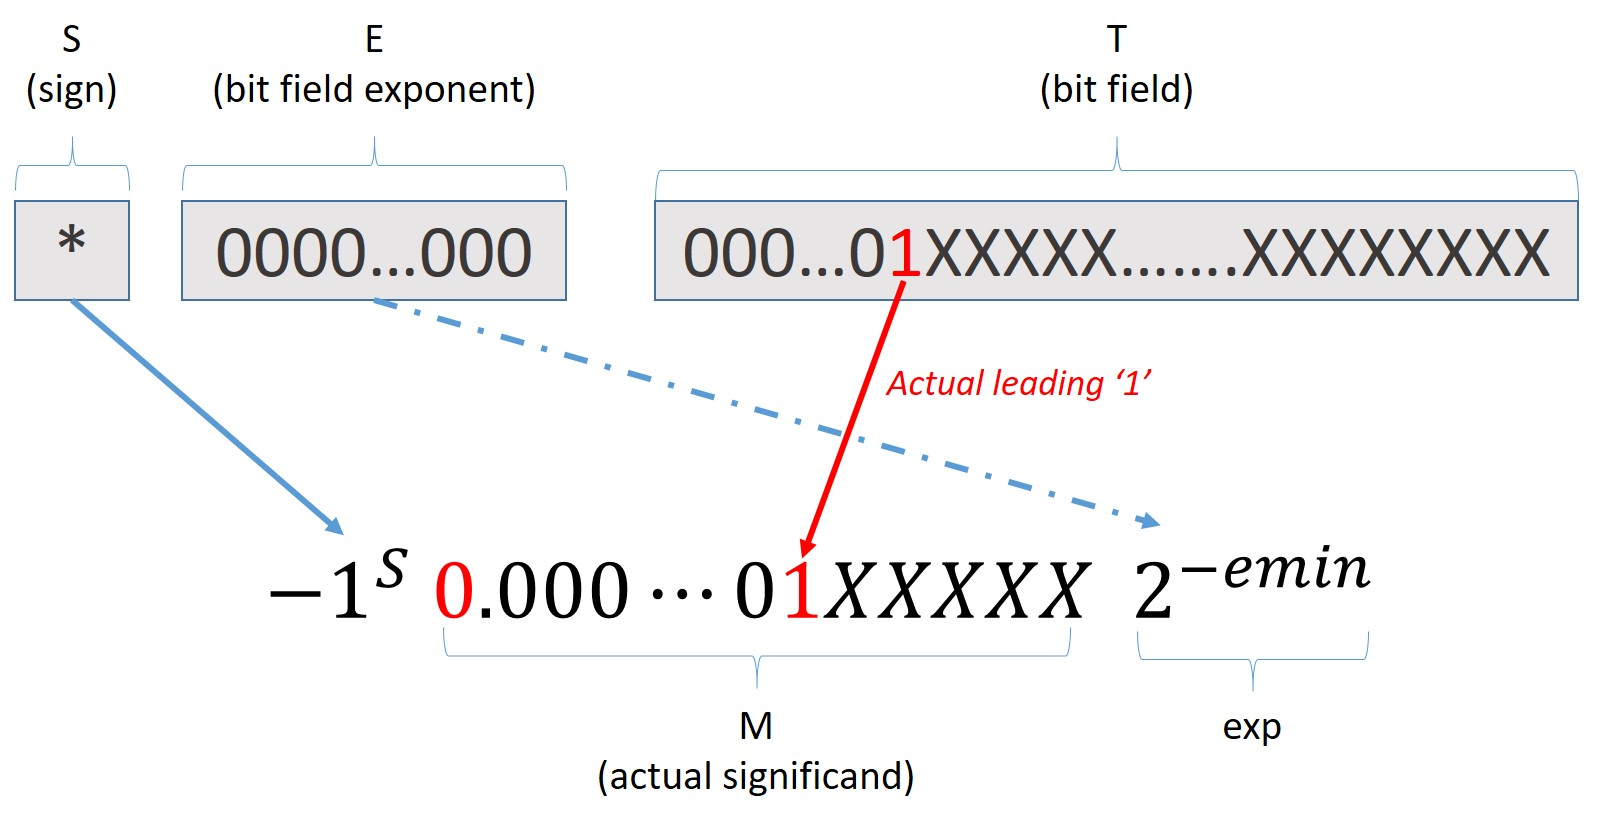
\includegraphics[scale=0.5]{subnormal}
  \caption{Subnormal representation.}
  \label{sybnormals}
\end{figure}

In the general case, we have $ 1 \leq M < 2 $ which guarantees that the representation is unique.
Since in the computer representation is finite, the exponent $exp$ can only have a finite range.  Therefore, a different rules applies for $M$ for numbers smaller than $ 1.0 \times 2^{emin}$. Those numbers are qualified as subnormals or denormals. In that case we have $ 0 < M < 1$ .

Practically, these numbers are differentiated by the encoding of field $E=0$. In that case, there is no implicit leading 1 for the mantissa:  the mantissa  stored in field T is considered with a leading 0.

\paragraph{Note:} supporting subnormals may be considered doubtful from the numerical analysis point of view, since it breaks the bound on representation relative error. However, it prevents the occurrence of underflow in subtraction. This is called gradual underflow because it allows a calculation to lose precision slowly when the result is small.

\subsection{NaNs}
\begin{itemize}[topsep=0pt]
\item If $E=2w-1$ and $T\neq 0$, the representation is a \emph{NaN} which means ``Not A Number''.
\end{itemize}
There are 2 different kinds of NaN, signaling and quiet. the most significant bit of the significand field determined whether a NaN is signaling or quiet : the value is non-zero if the NaN is quiet, and to zero if the NaN is signaling. \\
\begin{itemize}[topsep=0pt]
\item \textbf{Quiet NaNs} are used to propagate errors resulting from invalid operations or values such as overflow.
in IEEE 754, the underflow condition is only signaled if there is also a loss of precision.
\item \textbf{Signaling NaNs} can support advanced features such as mixing numerical and symbolic computation or other extensions to basic floating-point arithmetic.
\end{itemize}
% -----------------------------------------------
\section{Arithmetic Conformance}

\subsection{exactly rounded operations}
The IEEE standard requires that the result of addition, subtraction, multiplication, division, square-root, remainder, and conversion between integer and floating point formats be exactly rounded.


That is, the result must be equivalent as if computed exactly then rounded to the nearest floating-point number (using round to even). The Xvpfloat extension is only concened by exact rounding for addition, subtraction and multiplication.

\subsection{rounding rules}
The standard defines five rounding rules:
\begin{itemize}[topsep=0pt]
\item RNE: rounds to the nearest value; if the number falls midway, it is rounded to the nearest value with an even least significant digit; this is the default for binary floating point.
This corresponds to RNE rounding mode of Xvpfloat extension.
\item Round toward 0 : directed rounding towards zero (also known as truncation).
This corresponds to RTZ rounding mode of Xvpfloat extension.
\item Round toward $+\infty$  : directed rounding towards positive infinity (also known as rounding up or ceiling).
This corresponds to RUP rounding mode of Xvpfloat extension.
\item Round toward $-\infty$  : directed rounding towards negative infinity (also known as rounding down or floor).
This corresponds to RDN rounding mode of Xvpfloat extension.
\end{itemize}
These 4 modes are mandatory. The 5th rounding mode RNA is optional in radix 2, thus there is no necessity to implement it:
\begin{itemize}[topsep=0pt]
\item RNA:Round to nearest, ties away from zero : rounds to the nearest value. If the number falls midway, it is rounded to the nearest value above (for positive numbers) or below (for negative numbers).
This corresponds to RMM rounding mode of Xvpfloat extension.
\end{itemize}
At any time, one of the above four rounding modes is selected.
The programming environment should provide constants and functions for selecting (or alternatively reading) the active rounding mode dynamically in the course of a program (eg values such as \texttt{FE\_TONEAREST} or functions similar to C \emph{fesetround()}.

\paragraph{Note:} in theory, a modification of the rounding rule in a program should affect operations which appear after the change (in program order).

%% -----------------------------------------------
\section{Format configuration}

\subsection{From vpfloat language}
Within the vpfloat language, variables may be declared with constant size or dynamic size types, using the same declaration syntax, as shown in the fragment below :\\
\texttt{vpfloat<custom\_ieee, exp-info, bitsize-info> myVariable;} \\

Parameters exp-info and bit-info are integers which respectively represent the exponent and scalar bit sizes.

If exp-info and bitsize-info are not known at compile time, these parameters will be inferred at run time by a code fragment inserted at allocation time.

\paragraph{Important note:} a variable will be properly rounded to its actual significand size at store time.

\subsection{From Assembly language}
The Xvpfloat extension is only concerned about memory storage format during load and store operations.
Load and store operations will respectively decode and encode reals from/to memory according to the environment information stored in predefined registers \texttt{evp\textsubscript{i} and efp\textsubscript{i}}.
The concerned user environment is provided as an immediate in the instruction mnemonics \texttt{PLE}, \texttt{PLH}, \texttt{PLW} and \texttt{PLD} (resp \texttt{PSE}, \texttt{PSH}, \texttt{PSW} and \texttt{PSD}).

Each environment encodes following information about memory representation of variable precision numbers:
\begin{itemize}[topsep=0pt]
\item Exponent size (in bits).
\item Scalar variable footprint in memory (in bytes) is deduced from bit size rounded to the upper byte boundary.
\item Significand size (including implicit bit) is deduced from total footprint and exponent size.
\end{itemize}
There are up to 8 environments descriptors available for variable precision load/store instructions, and 8 more for half/float/double load/store instructions.
The exact behavior of load and store operations according to the environment is described in Section~\ref{sec:ls_ins}.
